%======================================================
% This file is part of
% "AMCOS_booklet"
% Version 1.1 (04/07/2019)
% A LaTeX template for conference books of abstracts
%
% This template is available at:
% https://github.com/maximelucas/AMCOS_booklet
%
% License: GNU General Public License v3.0
%
% Authors:
% Maxime Lucas (ml.maximelucas@gmail.com)
% Pau Clusella
%=======================================================

\documentclass[openany, parskip=full, 12pt, a4]{scrbook}

%======================================================
% This file is part of
% "AMCOS_booklet"
% Version 1.1 (04/07/2019)
% A LaTeX template for conference books of abstracts
%
% This template is available at:
% https://github.com/maximelucas/AMCOS_booklet
%
% License: GNU General Public License v3.0
%
% Authors:
% Maxime Lucas (ml.maximelucas@gmail.com)
% Pau Clusella
%=======================================================

\usepackage[utf8]{inputenc}
\usepackage[T1]{fontenc}
\usepackage{lmodern}

%---------------------------------------------------------
% PACKAGES
%---------------------------------------------------------

% TYPOGRAPHY
\usepackage{xspace}
\usepackage{microtype}
\usepackage{cmbright} % different fonts

% VARIA
\usepackage{color}
\usepackage[table]{xcolor} % loads also »colortbl« %load before tikz if options
\usepackage{scrhack} % fix koma script warning about addtolist
\usepackage{blindtext}
\usepackage{pdfpages} % for cover 
\usepackage{sectsty}

\usepackage{ifthen} % to have online and printed versionw

% GRAPHICS & FIGURES & TABLES
\usepackage{graphicx}
\usepackage{float}
\usepackage{multicol} % for timetable
\usepackage{longtable} % for list of participants over more than 1 page
% \usepackage[top=1.5cm, bottom=1.5cm, right=1.5cm, left=1.5cm]{geometry}
\usepackage[a4paper, margin=2.5cm]{geometry}
\usepackage{setspace}
%\usepackage{wrapfig}
%\usepackage{tikz}
%\tikzset{ar/.style={>=latex, ->}}
%\renewcommand{\arraystretch}{1.2}
%\usepackage[multidot]{grffile}
% \usepackage{booktabs}
\usepackage{caption}

% WANTS TO BE LAST
\usepackage[T1]{fontenc}
\usepackage[utf8]{inputenc}
%\usepackage[ngerman]{babel}
\usepackage[english]{babel}

\renewcommand{\contentsname}{Table of Contents} % Custom table of contents title

\subsectionfont{\large\color{myblue}\underline}  % sets colour of sections



\usepackage[hidelinks]{hyperref}
\hypersetup{pdfpagelayout=TwoPageRight}
% \usepackage[ocgcolorlinks]{hyperref}
% \hypersetup{colorlinks, linkcolor={wolf}, linktocpage=true, citecolor ={tpred}, urlcolor={black}}


%-------------------------------------------------------------
% SETTINGS
%-------------------------------------------------------------
\pagestyle{plain}

\setcounter{secnumdepth}{-2} % remove numbering at any level both for the heading and the toc
%https://tex.stackexchange.com/questions/30122/generate-table-of-contents-when-section-sections-without-numbering-has-been

%-------------------------------------------------------------
% USEFUL DEFINTIONS
%-------------------------------------------------------------

% VARIA 
\newcommand\tab[1][1cm]{\hspace*{#1}}


%======================================================
% This file is part of
% "AMCOS_booklet"
% Version 1.1 (04/07/2019)
% A LaTeX template for conference books of abstracts
%
% This template is available at:
% https://github.com/maximelucas/AMCOS_booklet
%
% License: GNU General Public License v3.0
%
% Authors:
% Maxime Lucas (ml.maximelucas@gmail.com)
% Pau Clusella
%=======================================================

%
% COLORS
%

\definecolor{myorange}{RGB}{255,117,40}
\definecolor{mygray}{RGB}{164, 168, 172}
\definecolor{mywhite}{RGB}{235, 238, 231}
\definecolor{myblue}{RGB}{52, 103, 103}

\newcommand{\primarycolor}{myblue}
\newcommand{\secondarycolor}{mywhite}
\newcommand{\ternarycolor}{mywhite}



\tolerance=1
\emergencystretch=\maxdimen
\hyphenpenalty=10000
\hbadness=10000

%
% BOOKLET VERSIONS
%

% If compilation is done with 'compile.sh', both versions (online and printed) are automatically compiled
% If compilation is done from editor, choose which version to compile below
\makeatletter
\@ifundefined{ifOnline}{% % check if already defined from the command line, if not define \ifOnline
	\expandafter\newif\csname ifOnline\endcsname
	\Onlinefalse %set to \Onlinefalse/\Onlinetrue for printed/online version
}{}
\makeatother

% define \type to input the right version of the abstracts
\ifOnline
\newcommand{\type}{o}
\else
\newcommand{\type}{p}
\fi % end if

%
% ABSTRACT ENVIRONMENTS
%

%----------------------------------------
% online abstract environment
%----------------------------------------
\newenvironment{symposium}[4] %{title}{author}{affiliation}{date}
{\filbreak %avoid page break
	
	{\large \bfseries \textcolor{myblue}{#1}}\newline\vspace{-10pt}\hrule

	{ \bfseries #3}
	\vspace{-10pt}

	{\bfseries \itshape Session chair(s): #2} 
	\vspace{-10pt}

	\textcolor{mygray}{#4}
	
}
{}

\newenvironment{abstract}[4] %{title}{author}{affiliation}{type}
{\filbreak %avoid page break
	
	{\large \bfseries #1}
	
	{\bfseries \itshape #2} 

	{#3}
	
	\textcolor{mygray}{#4}
	
}
{}

\newenvironment{keynote}[4] %{title}{author}{affiliation}{date}
{\filbreak %avoid page break
\begin{flushleft} \setstretch{1.5} 
	
	{\Huge \bfseries \textcolor{myblue}{#1}} 


\setstretch{1} 
\end{flushleft}

	{\large \bfseries \itshape #2}
	\vspace{-10pt}

	\textcolor{mygray}{#4} 

	{ \bfseries #3}\newline\hrule

	
}
{}


\newcommand{\poster}[3] %{title}{author}{affiliation}
{\filbreak %avoid page break
	
	{\bfseries \large #1} \\	
	\tab #2, \textit{#3}
	
}
{}

%----------------------------------------
% tags for talk type (colored circle in abstracts)
%----------------------------------------

\newcommand{\KLtag}{\tikz[baseline={([yshift=-.8ex]current bounding box.center)}]  \node[circle, inner sep=2pt, minimum size=0.5em, color=black, fill=\KLcolor]{\small \bfseries KL};} %colored circle with tag

\newcommand{\IStag}{\tikz[baseline={([yshift=-.8ex]current bounding box.center)}]  \node[circle, inner sep=2pt, minimum size=0.5em, color=black, fill=\IScolor]{\small \bfseries IS};} %colored circle with tag

\newcommand{\CTtag}{\tikz[baseline={([yshift=-.8ex]current bounding box.center)}]  \node[circle, inner sep=2pt, minimum size=0.5em, color=black, fill=\CTcolor]{\small \bfseries CT};} %colored circle with tag

\newcommand{\ITtag}{\tikz[baseline={([yshift=-.8ex]current bounding box.center)}]  \node[circle, inner sep=2pt, minimum size=0.5em, color=black, fill=\ITcolor]{\small \bfseries IT};} %colored circle with tag

%
% PAGE LAYOUT DEFINITIONS
%
\usepackage{etoolbox}

%------------------------------------------------------
% page style: vertical line on the side of each page
%------------------------------------------------------
\usepackage[scale=1,angle=0,opacity=1]{background}
\backgroundsetup{contents={}}

\AddEverypageHook{%
\ifthenelse{%
	\isodd{\thepage} \AND  \thepage>1 % if odd page but not front page
	}{%
	\backgroundsetup{
		color=\secondarycolor,
		position=current page.south east,%
		nodeanchor=south east,
		contents={\rule{10pt}{0.66\paperheight}}
		}
	}{%
	% nothing
	}
%
\ifthenelse{% 
	\NOT \isodd{\thepage} \AND \NOT \thepage=44% if even page
	}{%
	\backgroundsetup{
		color=\secondarycolor,
		position=current page.south west,%
		nodeanchor=south west,
		contents={\rule{10pt}{0.66\paperheight}}
		}
	}{%
	% nothing
	}
\BgMaterial}


%---------------------------------------------------
% chapter heading style
%---------------------------------------------------

\newdimen\mybarpadding
\mybarpadding=1.5em\relax %padding between gcolored bar and chapter name

\RedeclareSectionCommand[%
    ,afterskip=4em plus 1pt minus 1pt%
    ,beforeskip=-1pt%1.2em plus 1pt minus 1pt%
    ,level=0%
    ,toclevel=0%
]{chapter}%

\RedeclareSectionCommand[%
  afterindent=false,
  beforeskip=\baselineskip,
  afterskip=.5\baselineskip
]{section}%

\setkomafont{chapter}{\normalfont\normalsize\bfseries\Huge} % koma-script-specific command

\newcommand*{\mynumberedtest}[1]{% to test whether there is a number
  \if\relax\detokenize{#1}\relax%
  \else%
    #1%
    
  \fi}

%-------------------------------------------------chapter style definition

\renewcommand{\chapterlinesformat}[3]{%
  \Ifthispageodd{%
    \hfill%
    \raisebox{-0.2em}{%
      \makebox[0pt][r]{\textcolor{\primarycolor}{\rule{\paperwidth}{1em}}}%
    }%
    \hspace{\mybarpadding}%
% 	\mynumberedtest{#2}
	\mbox{#3}%
  }{%
%    \hbox{%
%       \mynumberedtest{#2}
      \mbox{#3}%
      \hspace{\mybarpadding}%
      \raisebox{-0.2em}{%
        \makebox[0pt][l]{\textcolor{\primarycolor}{\rule{\paperwidth}{1em}}}%
      }%
%    }%
  }%
}
\makeatother
%---------------------------------------------------------

% TIMETABLE COLORS AND STYLES

% text and backgroud colors
\newcommand{\tbg}{gray} % background
\newcommand{\tfg}{white}
\newcommand{\tbc}{gray!25}

% talk types colors
\newcommand{\IScolor}{myblue!65} % invited speaker
\newcommand{\CTcolor}{white} % contributed talk
\newcommand{\KLcolor}{myorange!45} % keynote lecture
\newcommand{\ITcolor}{yellow!25} %

% row types
\newcommand{\tablebreak}[2]{% {time span}{break name}
	\rowcolor{\tbc} #1 &  \multicolumn{4}{c|}{\bfseries #2} \\ \hline }
\newcommand{\eventtype}[2]{% {time span}{event name}
	#1& \multicolumn{4}{c|}{\cellcolor{\tbg}\color{\tfg}\bfseries #2} \\ \hline }

% column spacing and position
\newcolumntype{L}[1]{%
	>{\raggedright\let\newline\\\arraybackslash\hspace{0pt}}m{#1}}
\newcolumntype{C}[1]{%
	>{\centering\let\newline\\\arraybackslash\hspace{0pt}}m{#1}}
\newcolumntype{R}[1]{%
	>{\raggedleft\let\newline\\\arraybackslash\hspace{0pt}}m{#1}}

%\newcommand{\mytable}{|C{0.15\linewidth}| C{0.05\linewidth}|  C{0.25\linewidth} C{0.1\linewidth} C{0.5\linewidth}|}

\newcommand{\IS}[5]{% {time span}{name}{University}{City, Country}{title}
	#1 &\cellcolor{\IScolor}IS&{\bfseries#2}\newline #4&&#5 \\ \hline}
\newcommand{\CT}[5]{%
	#1 &\cellcolor{\CTcolor}CT&{\bfseries#2}\newline #4&&#5 \\ \hline}
\newcommand{\KL}[5]{%
	#1 &\cellcolor{\KLcolor}KL&{\bfseries#2}\newline #4&&#5 \\ \hline}
\newcommand{\IT}[5]{%
	#1 &\cellcolor{\ITcolor}IT&{\bfseries#2}\newline #4&&#5 \\ \hline}
\newcommand{\tutorial}[5]{%
	#1 && {\bfseries#2}\newline #4 &&#5 \\ \hline}



\usepackage{enumitem}
\setlist[description]{itemsep=-1ex, topsep=0.2pt}

	
\begin{document}


% COVER PAGE
%--------------------------------------------------------------------
% 
\includepdf{pdf_static/cover.pdf}	% our cover was produced with canva.com

	
	
% GENERAL INFORMATION
%---------------------------------------------------------------------
% \vspace*{1cm}
\begin{center}
	\textbf{GENERAL INFORMATION} \\
	\ \\[\baselineskip]

	\textcolor{\primarycolor}{\textbf{Host and Organisers}}	 \\
	Jan Born \\
	\ \\[\baselineskip]
	Max Harkotte \\
	Lisa Bastian \\
	Julia Fechner \\
	\ \\[\baselineskip]
	\vspace*{0.5cm}
	
	\textcolor{\primarycolor}{\textbf {Scientific Committee}}	 \\
	The Psychologie und Gehirn (PuG) 2023 conference is organised in close collaboration with the Fachgruppe Biologische Psychologie und Neuropsychologie of the German Psychological Association (DGPs) and the Deutsche Gesellschaft für Psychophysiologie und ihre Anwendung (DGPA). We thank both speakers, Prof. Hartwigsen (DGPs) and Prof. Hewig (DGPA), for their support in the scientific committee.
	\\[\baselineskip]
	\vspace*{0.5cm}

	\textcolor{\primarycolor}{\textbf {Contact}}	 \\
	\textbf{Website:} https://pug2023.de \\
	\textbf{E-Mail:} organisation@pug2023.de
	\\[\baselineskip]
	\vspace*{0.5cm}

	\textcolor{\primarycolor}{\textbf {Acknowledgementst}}	 \\
	We want to express our thanks to all sponsors for their invaluable financial support. Furthermore, we are grateful for the support of our student assistants in the run-up to the conference and their continuous support during the days of the meeting, ensuring that every question gets answered and every problem gets solved.

	PuG Logo Design by Katja Wahl (kwahl.de)

\end{center}
\mbox{}
\thispagestyle{empty}
\vfill
\begin{center}
	\ \\[20pt] % Please cite us by keeping the following line.
	The open-source \LaTeX{} template, AMCOS\_booklet, used to generate this booklet is available at \url{https://github.com/maximelucas/AMCOS\_booklet}
\end{center}

\newpage


% SPONSORS
%------------------------------------------------------------------
\chapter{Sponsors}
\begin{center}
We thank all our sponsors!
\end{center}

\vfill

\begin{center}
    \begin{tabular}{ c c }
        
\includegraphics[width=0.25\textwidth]{tex/images/sponsors/MES.png} & \hspace*{1cm} \vspace*{0.5cm}
        
\includegraphics[width=0.25\textwidth]{tex/images/sponsors/sr-research.png} \\ 
        
\includegraphics[width=0.25\textwidth]{tex/images/sponsors/Tecan.jpg} & \hspace*{1cm} \vspace*{0.5cm}
        
\includegraphics[width=0.25\textwidth]{tex/images/sponsors/easycap.png} \\ 
        
\includegraphics[width=0.25\textwidth]{tex/images/sponsors/mbt.png} & \hspace*{1cm} \vspace*{0.5cm}
        
\includegraphics[width=0.25\textwidth]{tex/images/sponsors/NIRx.png} \\ 
        \multicolumn{2}{c}{
\includegraphics[width=0.3\textwidth]{tex/images/sponsors/BFA.png}}     
    \end{tabular}
    \end{center}

\vfill

\newpage



% Welcome
%---------------------------------------------------------------------
\chapter{Welcome to Hamburg}
% Dear colleagues, or simply put: Moin!
 
It is with great pleasure that we welcome you to the 49th Annual Psychologie und Gehirn (PuG) Conference, which will be held at the Universität Hamburg and the Bürgerhaus Wilhelmsburg from May 29 to June 1, 2024. The PuG is jointly organized with the Fachgruppe Biologische Psychologie und Neuropsychologie (FGBPNP) der Deutschen Gesellschaft für Psychologie  (DGPs) und der Deutschen Gesellschaft für Psychophysiologie und ihre Anwendung (DGPA).
 
We are positively surprised (one might even say overwhelmed) by the huge interest in this year’s PuG conference, and proudly present a program that features a rich set of scientific and networking events, including pre-conference workshops (organized by the Early Career Researchers), 35 scientific symposia with about 150 talks, two poster sessions with over 400 posters, poster flash talks, a Buddy program as well as general assemblies of the organizing societies (DGPs, DGPA) and the Special Interest Group of Open and Reproducible Research (IGOR). Opening and social evenings at the Universität Hamburg and on the historic cargo ship Cap San Diego round off the program. The three keynote lectures given by Karin Roelofs, Katharina von Kriegstein, and Nils Kroemer will certainly be highlights of the conference.
 
We are thrilled to gather an international community of researchers to explore developments and foster collaborations in biological psychology, neuropsychology and adjacent fields. We especially look forward to facilitating meaningful dialogues and collaborations among researchers at all stages of their careers. Hosting this year's conference in Hamburg offers a unique setting known for its dynamic intersection of tradition and innovation. As a city that has long been a gateway to the world, Hamburg mirrors the spirit of discovery and connectivity that we aim to promote in our scientific discussions.
 
Looking forward to welcoming you to Hamburg for an inspiring assembly of minds and ideas!
 
Best regards, the local organizing team of PuG 2024:

Helen Blank, Patrick Bruns, Sebastian Gluth, Tina Lonsdorf, Anja Riesel, Brigitte Röder, Nico Schuck, Lars Schwabe, Jan Wacker

\newpage


% TABLE OF CONTENTS 
%---------------------------------------------------------------------
\tableofcontents


% USEFUL INFO
%------------------------------------------------------------------
\chapter{Useful Information}
% 
\setlength{\parskip}{1em}   

\section*{Conference site plan}

\begin{center}
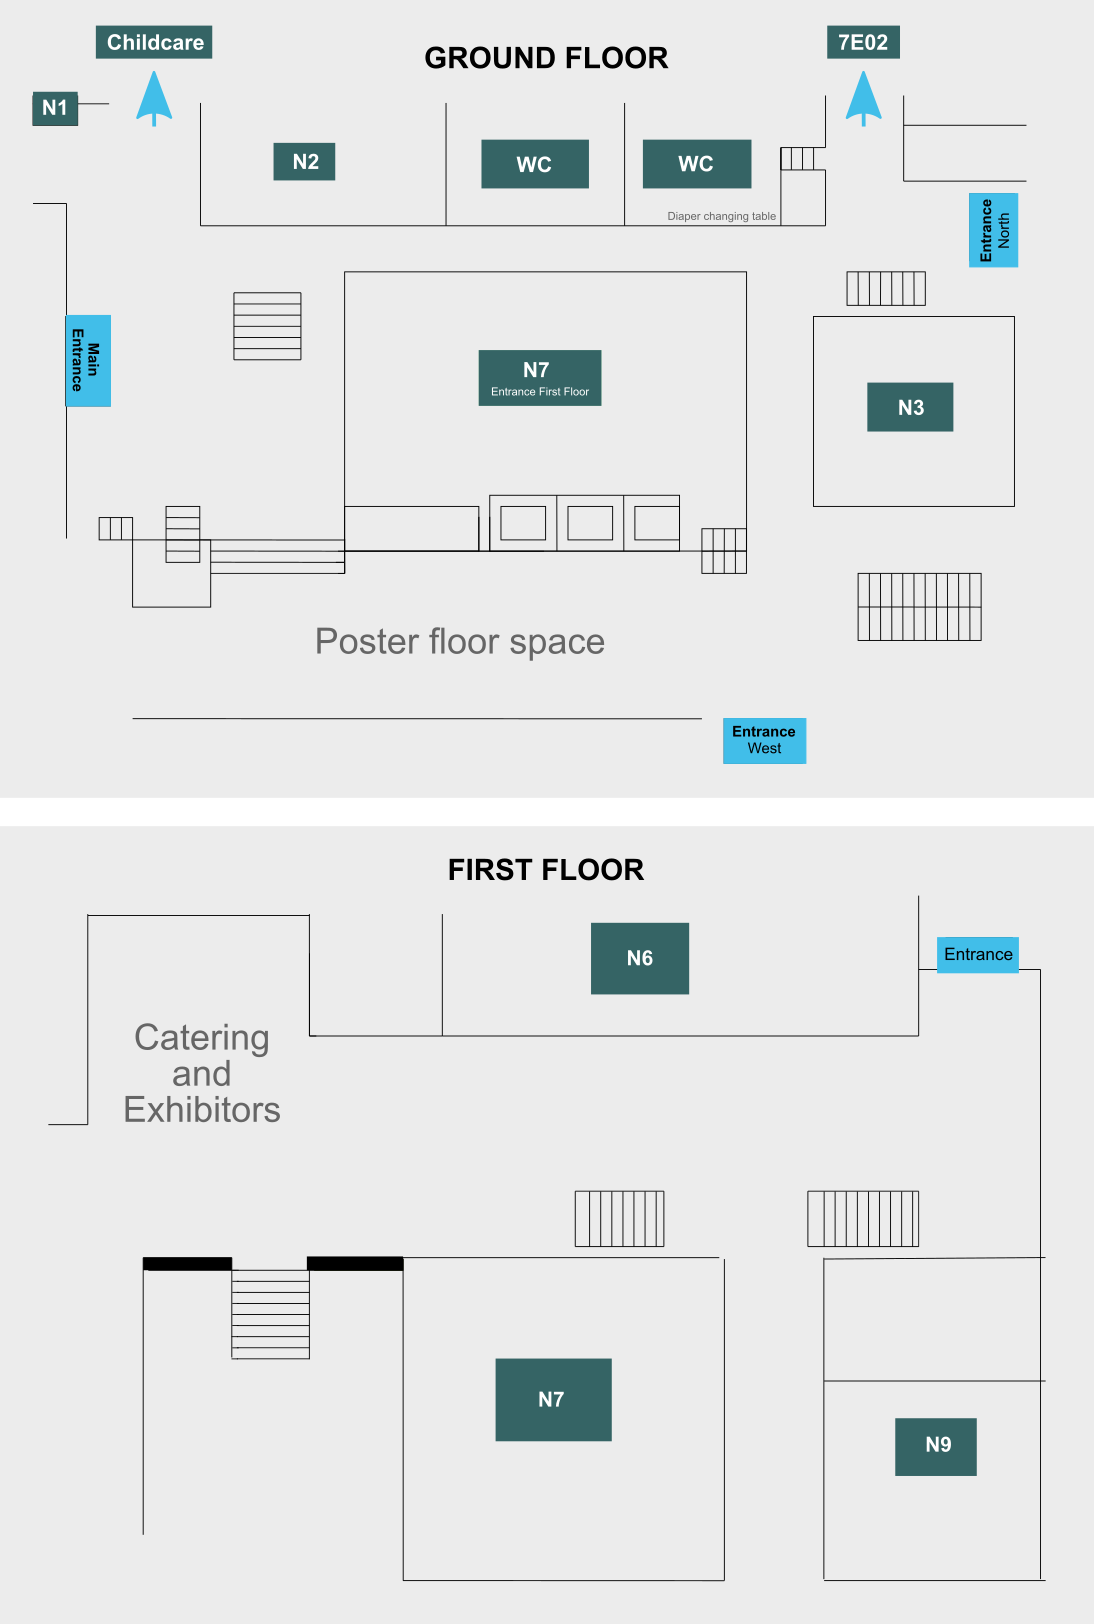
\includegraphics[width=0.8\textwidth]{tex/images/map.png}
\end{center}


\section*{How do I get to the venue?}

In general, we recommend the “Naldo” app, which will show you all the bus times in real time. Additionally, you can find all the bus lines online at https://www.swtue.de/oepnv/fahrplan-und-liniennetz/fahrplaene.html .

The closest bus stop to the venue is called “BG Unfallklinik” and is served by bus lines 5, 13, 14, 17, 18. Central bus stops in the city center are “Hauptbahnhof” (served by all bus lines), “Neckarbrücke” (served by 5, 13, 17, 18) and “Wilhelmstraße” (served by 5, 13, 17, 18).

If you stay in Reutlingen, train MEX 12, MEX 18, IRE 6 and RB 63 will bring you within 10 minutes to the main station in Tübingen. A train departs every half an hour.

\vspace*{-1cm}

\begin{center}
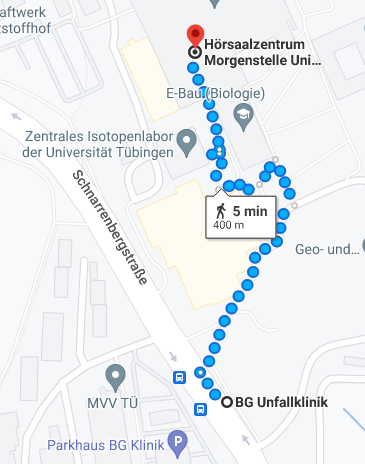
\includegraphics[width=0.5\textwidth]{tex/images/bus.png}
\end{center}

\section*{Accreditation}

Four symposia have been accredited by the Landespsychotherapeutenkammer Baden-Württembergwith with 2 credit points each. If you need a certificate of participation, ask our staff in the respective symposium session: 

\begin{itemize}
\setlength{\itemsep}{-0.8em} 
	\item S04 - Neurobiological Research to Optimize Therapeutic Interventions
	\item S16 - Computational Mechanisms of Learning and Decision-making in Psychiatry
	\item S20 - Prefrontal Cortical Function and Neuromodulation in Mental Disorders
	\item S36 - Deficits in Tactile Perception and their Clinical Implications
\end{itemize}

\section*{Childcare}

We offer childcare in the family room and if the weather is good also outside the conference center. Diaper changing tables can be found on the toilets. If you have any requests don't hesitate to get in touch at the front desk. 

\section*{How do I get to the social evening? And how do I get home later at night?}

The Brauwerk Freistil is located south of the Neckar and easily reachable from the main station or Neckarbrücke within 10 minutes by foot.

\begin{center}
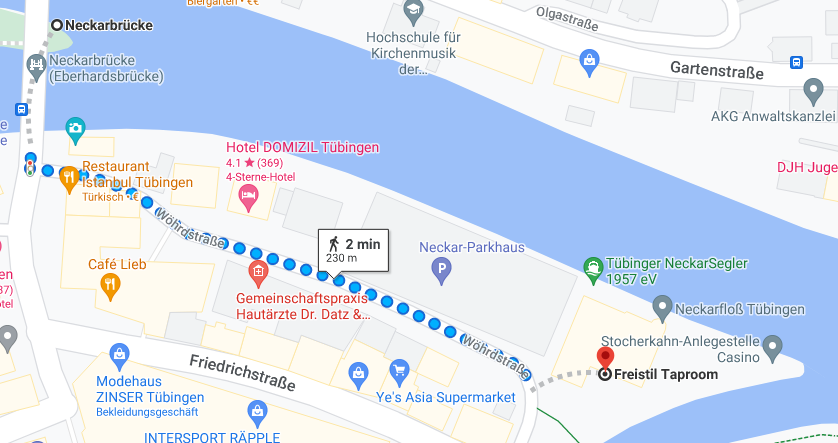
\includegraphics[width=1\textwidth]{tex/images/freistil.png}
\end{center}


Tübingen has a few night busses that run until 3 am. They are marked with an “N”. Alternatively, there are a few taxi companies:

\begin{itemize}
\setlength{\itemsep}{-0.8em} 
	\item Taxi Tübingen 07071 920555 and 0157 80989740
	\item Taxi Akublut 07071 1438591
	\item Taxi Maxi Tübingen 07071 7931064
	\item Taxi Easy 0173 1643229
\end{itemize}


\section*{What is a good place to eat and drink in Tübingen?}

Tübingen has a few nice cafés, restaurants and bars to offer. Coffee places with a nice atmosphere are Café Haag, Café Hanseatica, Willi Tübingen, Suedhang Kaffee and Katesch.
For authentic Swabian food, we recommend Krumme Brücke, Mauganeschtle, Marquardtei, Weinstube Forelle, Ratskeller and Wurstküche. The Neckarmüller is a nice beergarden and the Bären serves Swabian tapas! The Bären and Ratskeller are nice places to stay for one or a few more beers. Other good bars are the Jäger, Stadtpost, Chez Michel and the Irish pub Saints and Scholars.


\section*{And if I need money?}

Contactless payment is available almost everywhere, but some bars still rely on cash. You can find the nearest ATM close to the venue at the BG Klinik at Schnarrenbergstraße.

\begin{center}
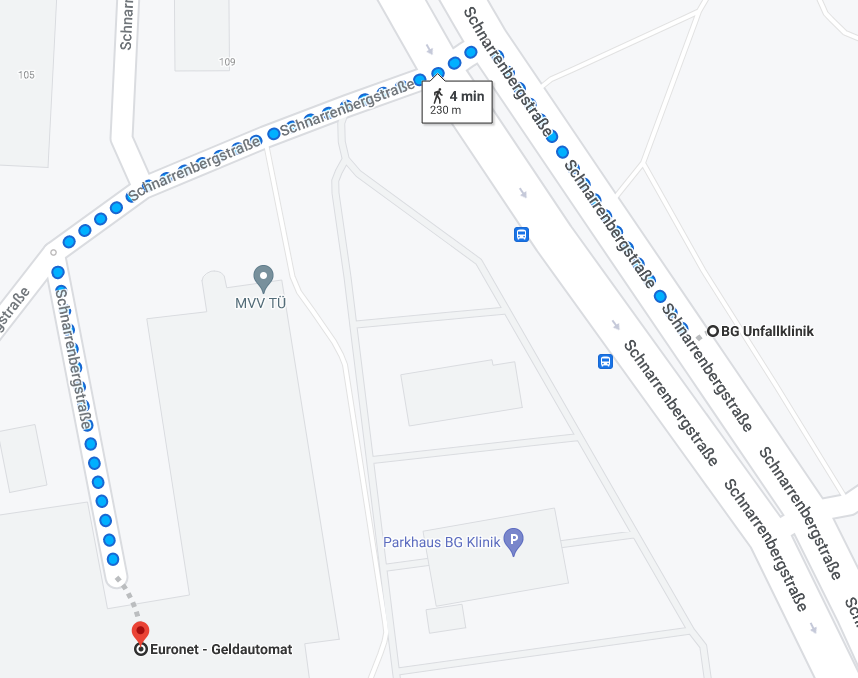
\includegraphics[width=0.8\textwidth]{tex/images/atm.png}
\end{center}


We hope that this information will make your stay as pleasant as possible and that you will enjoy the PuG in Tübingen to the fullest!




% TIMETABLE 
%---------------------------------------------------------------------
\chapter{Timetable}
% 
\section*{Welcome reception}
We are excited to start the PuG with you on Wednesday, 7th of June, at our welcoming evening! From 6 pm on, you can get your conference documents and register onsite at the front desk at the foyer of the Tagungszentrum Morgenstelle. The evening offers an opportunity for first encounters and to meet your fellow science colleagues. Live music provides a nice ambiance to enjoy free beer, soft drinks and vegetarian/vegan food.

\section*{Social evening}
We look forward to welcoming you to the social evening on Friday at Brauwerk Freistil! The Brauwerk is known for its home-brewed beers, which, unlike its industrial counterparts, make intense flavor experiences instead of simple thirst quenching a priority.

The entrance to the social evening begins directly after the conference program at 6:30 pm. International and local finger food (including vegan options), four free drinks and the beer garden directly at the Neckar are included in the ticket price of 80€. In addition, punting boats, an ice cream and a crepe truck will be provided for a summery ambience in the beer garden. Inside Freistil, you'll find a pool table, dart and shuffle boards, as well as a foosball table to compete against your colleagues. 

From 9:15 pm on there will be live performances by the PuG band and the latin american local band Combo Cumbiale. \textbf{In a short break at around 10 pm, we will award the Poster prizes, the IGOR prize and the prize for the best supervision.} The evening is rounded up by a live set of our DJ. 

Students and PhD students can purchase a party ticket for 35€ for the later part of the evening (entrance from 9:30 pm). Two free drinks are included in the ticket price.

\begin{center}
	
\includegraphics[width=0.3\textwidth]{tex/images/brauwerk.png}
\end{center}

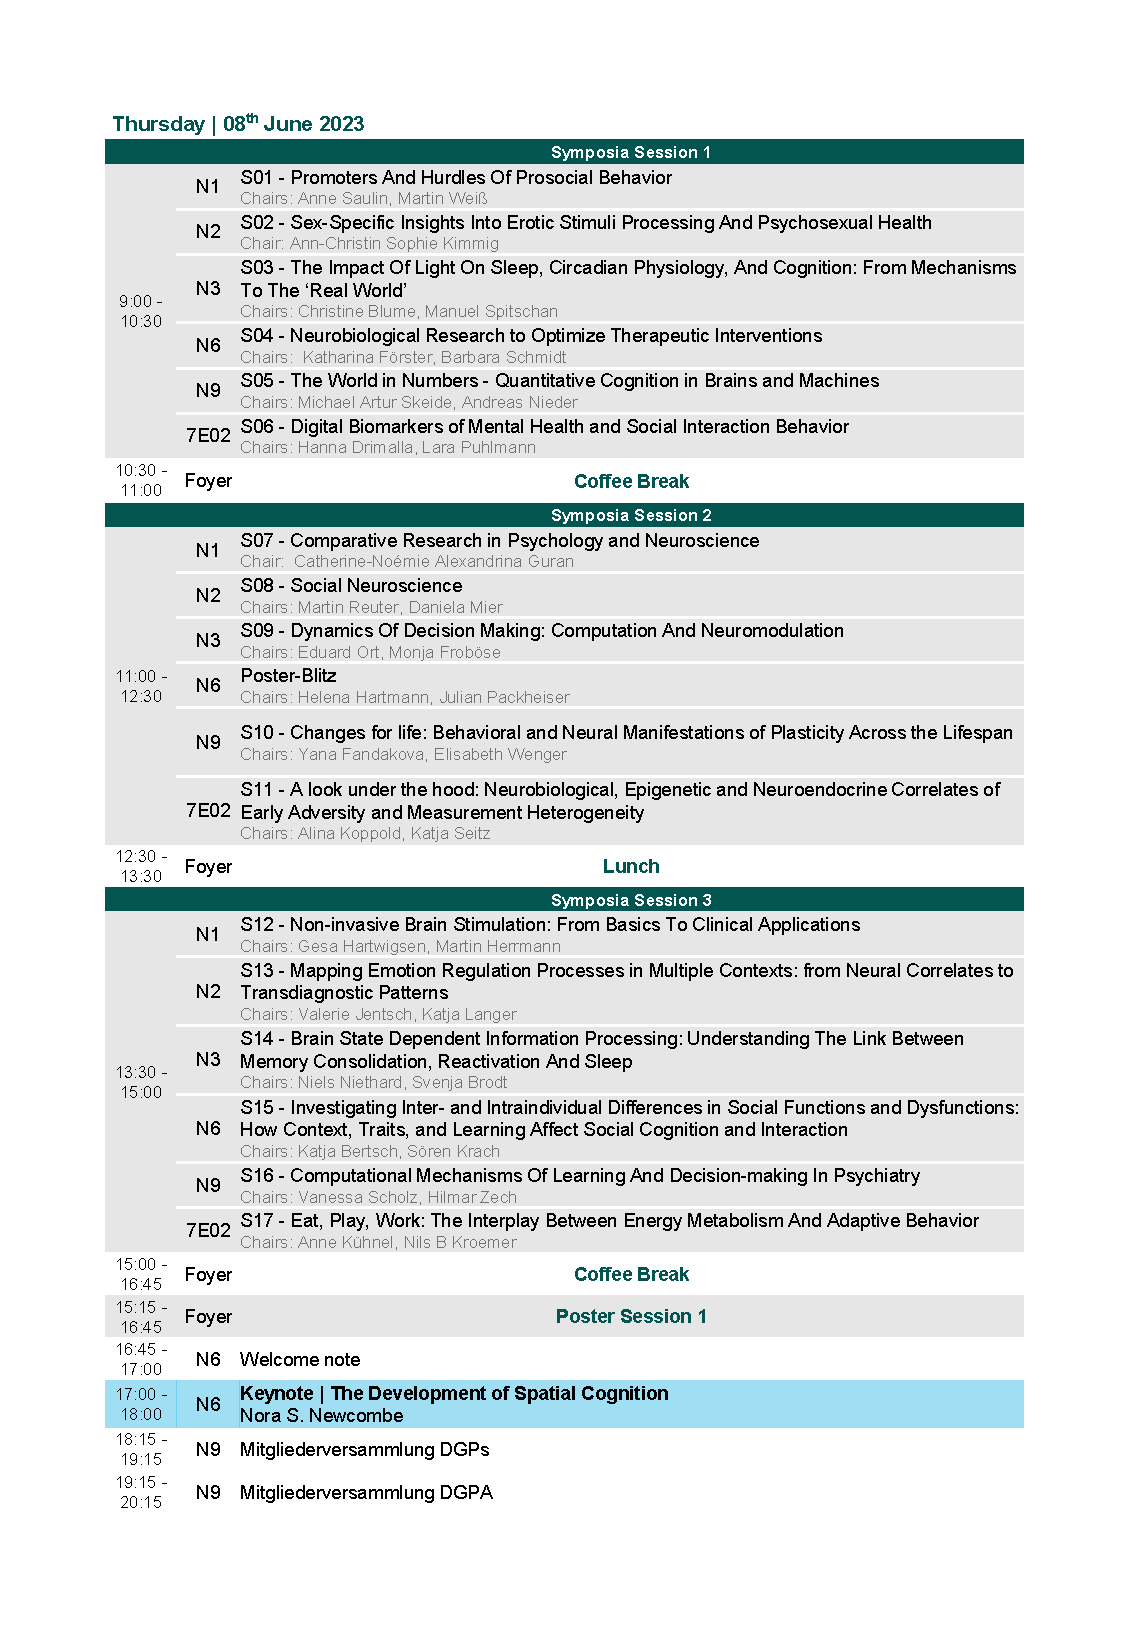
\includepdf[pages=-]{pdf_static/Program.pdf}
\includepdf[scale=0.8]{pdf_static/Social_Event_PuG}


% Definitions of custom environment used here can be found in preamble_booklet.tex file

% The following input commands automatically select the right version 
% (print or online) version of the abstract's .tex
% \type is defined in preamble_booklet.tex and equals:
% 'o' (online) or 'p' (print)


%Thursday
%---------------------------------------------------------------------
\chapter{Thursday | 30. May 2024}
\section{Keynote}
% \input{abstracts/tex/k_newcombe_form.tex}

\newpage

\section{Symposia session 1}

\begin{symposium}
{S01 - Exploring new approaches to increase utility of psychophysiological markers for clinical psychology}
{Session chair(s): Julia Klawohn, Hannes Per Carsten}
{Donnerstag 10:30 - 12:00 | Ort TODO}
{Welche Uni TODO}
Autor Julia Klawohn, Co-Autor: Hannes Per Carsten,

In recent years, biological markers have increasingly been incorporated into clinical research, showing they can further our knowledge of pathophysiological mechanisms underlying mental health problems and help identify new vantage points for interventions. Yet, despite these advances, limitations regarding robustness and effect sizes of associations between biological processes and clinical phenotypes remain and hamper practical utility of existing findings. This symposium will cover several studies that all attempt to improve bridging this gap by applying innovative experimental approaches or interventions, combining measures or methods, exploring underlying dimensions, or incorporating individualized materials. Kai Härpfer will present a large study spanning clinical and subclinical individuals, highlighting the importance of familial risk and lifetime diagnoses for variations in error-monitoring ERPs. Rosa Grützmann will show effects of a novel cognitive training aimed at reducing overactive error-processing in obsessive-compulsive disorder. She further demonstrates that a combination of several ERP markers can help improve diagnostic classification of mental health issues, like problematic internet use. Hannes Per Carsten extends the modification approach showing that VR-induced checking behavior may increase error-processing. Mareike Bayer presents a study combining EEG and fMRI to investigate emotional face processing in autism spectrum conditions, with results highlighting the importance of individualized stimuli. Finally, Julia Klawohn will show results indicating that emotional reactivity, as captured with both ERP and cardiac measures, can contribute to predictions of individual psychotherapy success in obsessive-compulsive disorder. Together, these findings capture the complexity of links between psychophysiological markers and psychopathology and propose leverage points for translational research strategies.
\begin{description}    

    \item [Kai Härpfer (TODO: refactor name)] TODO: add title \textcolor{mygray}{ | 10:30}    
    
    \item [Rosa Grützmann (TODO: refactor name)] TODO: add title \textcolor{mygray}{ | 10:45}    
    
    \item [Hannes Per Carsten (TODO: refactor name)] TODO: add title \textcolor{mygray}{ | 11:00}    
    
    \item [Mareike Bayer (TODO: refactor name)] TODO: add title \textcolor{mygray}{ | 11:15}    
    
    \item [Julia Klawohn  (TODO: refactor name)] TODO: add title \textcolor{mygray}{ | 11:30}    
    
\end{description} 
\end{symposium}

% \input{abstracts/tex/s_S02_kimmig.tex}
% \input{abstracts/tex/s_S03_blume.tex}
% \input{abstracts/tex/s_S04_foerster_form.tex}
% \input{abstracts/tex/s_S05_skeide.tex}
% \input{abstracts/tex/s_S06_drimalla.tex}

\newpage

\section{Symposia session 2}
% \input{abstracts/tex/s_S07_guran.tex}
% \input{abstracts/tex/s_S08_reuter.tex}
% \input{abstracts/tex/s_S09_ort.tex}
% \input{abstracts/tex/s_posterblitz.tex}
% \input{abstracts/tex/s_S10_fandakova.tex}
% \input{abstracts/tex/s_S11_koppold_form.tex}

\newpage

\section{Symposia session 3}
% \input{abstracts/tex/s_S12_hartwigsen.tex}
% \input{abstracts/tex/s_S13_jentsch.tex}
% \input{abstracts/tex/s_S14_niethard_form.tex}
% \input{abstracts/tex/s_S15_bertsch.tex}
% \input{abstracts/tex/s_S16_scholz.tex}
% \input{abstracts/tex/s_S17_kuehnel.tex}

\newpage

\section{Poster session 1 }

\subsection*{Computational Methods and Neuroimaging}

% \input{abstracts/tex/pshort_199_metzen.tex}
% \input{abstracts/tex/pshort_207_tuzsus.tex}
% \input{abstracts/tex/pshort_214_goltermann.tex}
% \input{abstracts/tex/pshort_217_nold.tex}
% \input{abstracts/tex/pshort_222_garlichs.tex}
% \input{abstracts/tex/pshort_259_klapprott.tex}
% \input{abstracts/tex/pshort_295_schwarz.tex}
% \input{abstracts/tex/pshort_296_dellert.tex}
% \input{abstracts/tex/pshort_353_wolber.tex}
% \input{abstracts/tex/pshort_354_farshad.tex}
% \input{abstracts/tex/pshort_452_pinger.tex}

\subsection*{Individual Differences and (Epi)Genetics}

% \input{abstracts/tex/pshort_163_vetterlein.tex}
% \input{abstracts/tex/pshort_191_zerna.tex}
% \input{abstracts/tex/pshort_216_schiller.tex}
% \input{abstracts/tex/pshort_246_stein.tex}
% \input{abstracts/tex/pshort_271_keppler.tex}
% \input{abstracts/tex/pshort_290_fricke.tex}
% \input{abstracts/tex/pshort_310_kouris.tex}
% \input{abstracts/tex/pshort_318_geissert.tex}
% \input{abstracts/tex/pshort_327_popp.tex}
% \input{abstracts/tex/pshort_349_wehrheim.tex}


\subsection*{Learning, Memory, and Sleep}

% \input{abstracts/tex/pshort_125_joechner.tex}
% \input{abstracts/tex/pshort_165_bledowski.tex}
% \input{abstracts/tex/pshort_183_pavlov.tex}
% \input{abstracts/tex/pshort_186_ruettgens.tex}
% \input{abstracts/tex/pshort_190_alcan.tex}
% \input{abstracts/tex/pshort_197_wallenwein.tex}
% \input{abstracts/tex/pshort_201_nolting.tex}
% \input{abstracts/tex/pshort_244_zoellner.tex}
% \input{abstracts/tex/pshort_267_palmieri.tex}
% \input{abstracts/tex/pshort_278_kern.tex}
% \input{abstracts/tex/pshort_312_butavand.tex}
% \input{abstracts/tex/pshort_317_soldan.tex}
% \input{abstracts/tex/pshort_329_poetzl.tex}
% \input{abstracts/tex/pshort_335_schaefer.tex}
% \input{abstracts/tex/pshort_337_teng.tex}
% \input{abstracts/tex/pshort_340_wuest.tex}
% \input{abstracts/tex/pshort_341_zhozhikashvili.tex}
% \input{abstracts/tex/pshort_345_plog.tex}
% \input{abstracts/tex/pshort_351_caviola.tex}
% \input{abstracts/tex/pshort_359_grassi.tex}
% \input{abstracts/tex/pshort_369_kumral.tex}
% \input{abstracts/tex/pshort_372_hainke.tex}
% \input{abstracts/tex/pshort_374_wernicke.tex}
% \input{abstracts/tex/pshort_381_kutlu.tex}
% \input{abstracts/tex/pshort_382_hahn.tex}
% \input{abstracts/tex/pshort_510_fischer.tex}
% \input{abstracts/tex/pshort_521_nagel.tex}
% \input{abstracts/tex/pshort_534_lauckner.tex}
% \input{abstracts/tex/pshort_544_janssen.tex}

\subsection*{Cognition}

% \input{abstracts/tex/pshort_156_iwama.tex}
% \input{abstracts/tex/pshort_164_thiele.tex}
% \input{abstracts/tex/pshort_166_rodrigues.tex}
% \input{abstracts/tex/pshort_171_papin.tex}
% \input{abstracts/tex/pshort_172_tast.tex}
% \input{abstracts/tex/pshort_212_eymann.tex}
% \input{abstracts/tex/pshort_248_potamianou.tex}
% \input{abstracts/tex/pshort_251_schmidt.tex}
% \input{abstracts/tex/pshort_275_lange.tex}
% \input{abstracts/tex/pshort_291_porth.tex}
% \input{abstracts/tex/pshort_344_asan.tex}
% \input{abstracts/tex/pshort_373_kurtenbach.tex}
% \input{abstracts/tex/pshort_377_golowin.tex}
% \input{abstracts/tex/pshort_379_maile.tex}
% \input{abstracts/tex/pshort_384_albrecht.tex}
% \input{abstracts/tex/pshort_506_bittner.tex}
% \input{abstracts/tex/pshort_514_kanatschnig.tex}
% \input{abstracts/tex/pshort_542_wendiggensen.tex}
% \input{abstracts/tex/pshort_644_kang.tex}

\subsection*{Attention and Perception}

% \input{abstracts/tex/pshort_101_menger.tex}
% \input{abstracts/tex/pshort_195_roeber.tex}
% \input{abstracts/tex/pshort_215_wang.tex}
% \input{abstracts/tex/pshort_263_raposo.tex}
% \input{abstracts/tex/pshort_270_kisker.tex}
% \input{abstracts/tex/pshort_298_garridovasquez.tex}
% \input{abstracts/tex/pshort_333_wu.tex}
% \input{abstracts/tex/pshort_364_dimigen.tex}
% \input{abstracts/tex/pshort_393_mueller.tex}
% \input{abstracts/tex/pshort_395_tholl.tex}
% \input{abstracts/tex/pshort_407_ayatollahi.tex}

\subsection*{Brain and Periphery, Neuroendocrinology, and Stress}

% \input{abstracts/tex/pshort_107_berretz.tex}
% \input{abstracts/tex/pshort_213_schmidt.tex}
% \input{abstracts/tex/pshort_223_matits.tex}
% \input{abstracts/tex/pshort_226_tiemann.tex}
% \input{abstracts/tex/pshort_261_henze.tex}
% \input{abstracts/tex/pshort_265_lashani.tex}
% \input{abstracts/tex/pshort_299_huthsteiner.tex}
% \input{abstracts/tex/pshort_315_knopf.tex}
% \input{abstracts/tex/pshort_319_schwarze.tex}
% \input{abstracts/tex/pshort_328_lipka.tex}
% \input{abstracts/tex/pshort_330_rosada.tex}
% \input{abstracts/tex/pshort_361_wolsink.tex}
% \input{abstracts/tex/pshort_366_linnig.tex}
% \input{abstracts/tex/pshort_387_raduenz.tex}
% \input{abstracts/tex/pshort_424_matthaeus.tex}
% \input{abstracts/tex/pshort_590_degering.tex}
% \input{abstracts/tex/pshort_594_bernard.tex}
% \input{abstracts/tex/pshort_606_kollmann.tex}

\subsection*{Social and Environmental Neuroscience}

% \input{abstracts/tex/pshort_255_maier.tex}
% \input{abstracts/tex/pshort_258_ocklenburg.tex}
% \input{abstracts/tex/pshort_262_gado.tex}
% \input{abstracts/tex/pshort_272_yang.tex}
% \input{abstracts/tex/pshort_281_mitschke.tex}
% \input{abstracts/tex/pshort_289_maria.tex}
% \input{abstracts/tex/pshort_292_sagehorn.tex}
% \input{abstracts/tex/pshort_293_schneider.tex}
% \input{abstracts/tex/pshort_305_haerpfer.tex}
% \input{abstracts/tex/pshort_309_korte.tex}
% \input{abstracts/tex/pshort_339_kogler.tex}
% \input{abstracts/tex/pshort_348_berti.tex}
% \input{abstracts/tex/pshort_389_zhang.tex}
% \input{abstracts/tex/pshort_574_meller.tex}
% \input{abstracts/tex/pshort_593_manivasagam.tex}
\newpage

\subsection*{Development and Ageing}

% \input{abstracts/tex/pshort_158_semeia.tex}
% \input{abstracts/tex/pshort_232_kraemer.tex}
% \input{abstracts/tex/pshort_355_marx.tex}
% \input{abstracts/tex/pshort_356_klingelhoeferjens.tex}
% \input{abstracts/tex/pshort_409_enge.tex}
% \input{abstracts/tex/pshort_563_ghorbani.tex}
% \input{abstracts/tex/pshort_567_maydych.tex}

\subsection*{Disorders and Interventions}

% \input{abstracts/tex/pshort_211_hitzler.tex}
% \input{abstracts/tex/pshort_236_marek.tex}
% \input{abstracts/tex/pshort_239_staechele.tex}
% \input{abstracts/tex/pshort_250_anthes.tex}
% \input{abstracts/tex/pshort_266_lieberz.tex}
% \input{abstracts/tex/pshort_287_munoz.tex}
% \input{abstracts/tex/pshort_294_bayer.tex}
% \input{abstracts/tex/pshort_304_bayer.tex}
% \input{abstracts/tex/pshort_323_esser.tex}
% \input{abstracts/tex/pshort_324_lottsandkamp.tex}
% \input{abstracts/tex/pshort_331_abdoust.tex}
% \input{abstracts/tex/pshort_342_gruzman.tex}
% \input{abstracts/tex/pshort_362_graumann.tex}
% \input{abstracts/tex/pshort_365_hempel.tex}
% \input{abstracts/tex/pshort_391_illius.tex}
% \input{abstracts/tex/pshort_392_meier.tex}
% \input{abstracts/tex/pshort_414_halli.tex}
% \input{abstracts/tex/pshort_421_eder.tex}

\subsection*{(Brain) Stimulation}

% \input{abstracts/tex/pshort_252_weber.tex}
% \input{abstracts/tex/pshort_282_woehrstein.tex}
% \input{abstracts/tex/pshort_334_niessen.tex}
% \input{abstracts/tex/pshort_410_fromm.tex}
% \input{abstracts/tex/pshort_418_geisler.tex}

\subsection*{Affective Neuroscience}

% \input{abstracts/tex/pshort_160_packheiser.tex}
% \input{abstracts/tex/pshort_219_bierbrauer.tex}
% \input{abstracts/tex/pshort_220_witte.tex}
% \input{abstracts/tex/pshort_237_pfeifer.tex}
% \input{abstracts/tex/pshort_240_wuest.tex}
% \input{abstracts/tex/pshort_242_dietrich.tex}
% \input{abstracts/tex/pshort_249_konrad.tex}
% \input{abstracts/tex/pshort_260_teigeler.tex}
% \input{abstracts/tex/pshort_280_goeller.tex}
% \input{abstracts/tex/pshort_308_wurtz.tex}
% \input{abstracts/tex/pshort_358_lingelbach.tex}
% \input{abstracts/tex/pshort_445_singhi.tex}

\subsection*{Open, Reproducable and Meta Science}

% \input{abstracts/tex/pshort_178_gaertner.tex}
% \input{abstracts/tex/pshort_371_luebber.tex}
% \input{abstracts/tex/pshort_405_zhang.tex}
% \input{abstracts/tex/pshort_505_stute.tex}
% \input{abstracts/tex/pshort_599_doerfel.tex}
\newpage



%Friday
%---------------------------------------------------------------------
\chapter{Friday | 31. May 2024}
% 
\section{Keynote}
\input{abstracts/tex/k_sandi_form.tex}

\newpage

\section{Symposia session 4}
\input{abstracts/tex/s_S18_thiel_form.tex}
\input{abstracts/tex/s_S19_reutter.tex}
\input{abstracts/tex/s_S20_barth.tex}
\input{abstracts/tex/s_S21_morawetz.tex}
\input{abstracts/tex/s_S22_rufener.tex}
\newpage

\section{Symposia session 5}
\input{abstracts/tex/s_S23_kastrinogiannis_form.tex}
\input{abstracts/tex/s_S24_mueller.tex}
\input{abstracts/tex/s_panel.tex}
\input{abstracts/tex/s_S25_feld.tex}
\input{abstracts/tex/s_S26_weidner.tex}

\newpage

\section{Symposia session 6}
\input{abstracts/tex/s_S27_weber.tex}
\input{abstracts/tex/s_S28_stock.tex}
\input{abstracts/tex/s_S29_paulus.tex}
\input{abstracts/tex/s_S30_jacobsen.tex}
\input{abstracts/tex/s_S31_paulus.tex}
\newpage

\section{Poster session 2}

\subsection*{Computational Methods and Neuroimaging}

\input{abstracts/tex/pshort_480_haugg.tex}
\input{abstracts/tex/pshort_488_kraljevic.tex}
\input{abstracts/tex/pshort_491_nowaczynski.tex}
\input{abstracts/tex/pshort_522_samuel.tex}
\input{abstracts/tex/pshort_531_boettcher.tex}
\input{abstracts/tex/pshort_539_kober.tex}
\input{abstracts/tex/pshort_546_schulz.tex}
\input{abstracts/tex/pshort_548_guersoy.tex}
\input{abstracts/tex/pshort_575_zhang.tex}
\input{abstracts/tex/pshort_614_ershadmanesh.tex}
\input{abstracts/tex/pshort_624_goltermann.tex}

\subsection*{Individual Differences and (Epi)Genetics}

\input{abstracts/tex/pshort_241_wuest.tex}
\input{abstracts/tex/pshort_376_schmidt.tex}
\input{abstracts/tex/pshort_386_mack.tex}
\input{abstracts/tex/pshort_413_wegrzyn.tex}
\input{abstracts/tex/pshort_458_goeller.tex}
\input{abstracts/tex/pshort_486_lang.tex}
\input{abstracts/tex/pshort_543_nazarenus.tex}
\input{abstracts/tex/pshort_556_rafiee.tex}
\input{abstracts/tex/pshort_571_usemann.tex}
\input{abstracts/tex/pshort_647_jawinski.tex}

\subsection*{Learning, Memory, and Sleep}

\input{abstracts/tex/pshort_184_pavlov.tex}
\input{abstracts/tex/pshort_433_wick.tex}
\input{abstracts/tex/pshort_434_baselgia.tex}
\input{abstracts/tex/pshort_444_rauss.tex}
\input{abstracts/tex/pshort_449_li.tex}
\input{abstracts/tex/pshort_464_luettgau.tex}
\input{abstracts/tex/pshort_496_lutz.tex}
\input{abstracts/tex/pshort_537_dabas.tex}
\input{abstracts/tex/pshort_545_cybinski.tex}
\input{abstracts/tex/pshort_552_lenders.tex}
\input{abstracts/tex/pshort_553_kleespies.tex}
\input{abstracts/tex/pshort_566_arslan.tex}
\input{abstracts/tex/pshort_568_kasties.tex}
\input{abstracts/tex/pshort_570_sawangjit.tex}
\input{abstracts/tex/pshort_573_uelkue.tex}
\input{abstracts/tex/pshort_583_biel.tex}
\input{abstracts/tex/pshort_585_klatt.tex}
\input{abstracts/tex/pshort_586_johnsdorf.tex}
\input{abstracts/tex/pshort_589_nguyen.tex}
\input{abstracts/tex/pshort_602_weber.tex}
\input{abstracts/tex/pshort_603_ameen.tex}
\input{abstracts/tex/pshort_604_schmidt.tex}
\input{abstracts/tex/pshort_608_sayk.tex}
\input{abstracts/tex/pshort_618_ehsanifard.tex}
\input{abstracts/tex/pshort_622_kampa.tex}
\input{abstracts/tex/pshort_628_hinterberger.tex}
\input{abstracts/tex/pshort_632_eigl.tex}
\input{abstracts/tex/pshort_651_klein.tex}

\subsection*{Cognition}

\input{abstracts/tex/pshort_451_paul.tex}
\input{abstracts/tex/pshort_503_schroeder.tex}
\input{abstracts/tex/pshort_525_brands.tex}
\input{abstracts/tex/pshort_527_anwander.tex}
\input{abstracts/tex/pshort_551_lembke.tex}
\input{abstracts/tex/pshort_558_reinke.tex}
\input{abstracts/tex/pshort_564_mattes.tex}
\input{abstracts/tex/pshort_572_taylor.tex}
\input{abstracts/tex/pshort_577_noll.tex}
\input{abstracts/tex/pshort_578_prochnow.tex}
\input{abstracts/tex/pshort_581_nebe.tex}
\input{abstracts/tex/pshort_587_wilken.tex}
\input{abstracts/tex/pshort_588_kolano.tex}
\input{abstracts/tex/pshort_596_algermissen.tex}
\input{abstracts/tex/pshort_598_mueckstein.tex}
\input{abstracts/tex/pshort_611_reicherts.tex}
\input{abstracts/tex/pshort_615_bellebaum.tex}
\input{abstracts/tex/pshort_617_ershadmanesh.tex}
\input{abstracts/tex/pshort_630_langner.tex}
\input{abstracts/tex/pshort_633_jueres.tex}
\input{abstracts/tex/pshort_634_bechtold.tex}

\subsection*{Attention and Perception}

\input{abstracts/tex/pshort_472_giron.tex}
\input{abstracts/tex/pshort_479_vigh.tex}
\input{abstracts/tex/pshort_484_quirmbach.tex}
\input{abstracts/tex/pshort_493_czernochowski.tex}
\input{abstracts/tex/pshort_499_terlau.tex}
\input{abstracts/tex/pshort_529_egan.tex}
\input{abstracts/tex/pshort_530_boettcher.tex}
\input{abstracts/tex/pshort_579_prochnow.tex}
\input{abstracts/tex/pshort_584_truong.tex}

\subsection*{Brain and Periphery, Neuroendocrinology, and Stress}

\input{abstracts/tex/pshort_436_vogel.tex}
\input{abstracts/tex/pshort_438_akan.tex}
\input{abstracts/tex/pshort_447_haase.tex}
\input{abstracts/tex/pshort_453_schindler.tex}
\input{abstracts/tex/pshort_463_omalley.tex}
\input{abstracts/tex/pshort_497_klink.tex}
\input{abstracts/tex/pshort_517_schmidtkassow.tex}
\input{abstracts/tex/pshort_519_buntic.tex}
\input{abstracts/tex/pshort_547_planert.tex}
\input{abstracts/tex/pshort_550_sperl.tex}
\input{abstracts/tex/pshort_559_boegemann.tex}
\input{abstracts/tex/pshort_565_blaser.tex}
\input{abstracts/tex/pshort_569_hansen.tex}
\input{abstracts/tex/pshort_620_haugwitz.tex}
\input{abstracts/tex/pshort_621_larra.tex}
\input{abstracts/tex/pshort_625_drost.tex}
\input{abstracts/tex/pshort_631_mueller.tex}
\input{abstracts/tex/pshort_639_heinrichs.tex}
\input{abstracts/tex/pshort_640_boehme.tex}
\input{abstracts/tex/pshort_641_lorusso.tex}

\subsection*{Social and Environmental Neuroscience}

\input{abstracts/tex/pshort_426_denk.tex}
\input{abstracts/tex/pshort_432_ambrase.tex}
\input{abstracts/tex/pshort_457_maliske.tex}
\input{abstracts/tex/pshort_465_korn.tex}
\input{abstracts/tex/pshort_471_kupersmith.tex}
\input{abstracts/tex/pshort_501_eisenbarth.tex}
\input{abstracts/tex/pshort_508_peters.tex}
\input{abstracts/tex/pshort_523_oswald.tex}
\input{abstracts/tex/pshort_535_kroll.tex}
\input{abstracts/tex/pshort_562_huang.tex}
\input{abstracts/tex/pshort_591_hopf.tex}
\input{abstracts/tex/pshort_595_fischer.tex}
\input{abstracts/tex/pshort_609_clusmann.tex}
\input{abstracts/tex/pshort_616_szeska.tex}
\input{abstracts/tex/pshort_643_lehmann.tex}
\input{abstracts/tex/pshort_648_daeglau.tex}

\subsection*{Development and Ageing}

\input{abstracts/tex/pshort_448_buritica.tex}
\input{abstracts/tex/pshort_450_meyer.tex}
\input{abstracts/tex/pshort_466_jockwitz.tex}
\input{abstracts/tex/pshort_474_ruge.tex}
\input{abstracts/tex/pshort_485_gaertner.tex}
\input{abstracts/tex/pshort_536_sturgeon.tex}
\input{abstracts/tex/pshort_636_dierolf.tex}

\subsection*{Disorders and Interventions}

\input{abstracts/tex/pshort_159_kudielka.tex}
\input{abstracts/tex/pshort_209_sahm.tex}
\input{abstracts/tex/pshort_439_schulz.tex}
\input{abstracts/tex/pshort_478_klepzig.tex}
\input{abstracts/tex/pshort_487_dastgheib.tex}
\input{abstracts/tex/pshort_509_fascher.tex}
\input{abstracts/tex/pshort_513_loeloff.tex}
\input{abstracts/tex/pshort_518_gehlen.tex}
\input{abstracts/tex/pshort_524_carsten.tex}
\input{abstracts/tex/pshort_532_korkmaz.tex}
\input{abstracts/tex/pshort_533_balzus.tex}
\input{abstracts/tex/pshort_538_peters.tex}
\input{abstracts/tex/pshort_540_meiering.tex}
\input{abstracts/tex/pshort_549_schulz.tex}
\input{abstracts/tex/pshort_554_boegl.tex}
\input{abstracts/tex/pshort_557_unternaehrer.tex}
\input{abstracts/tex/pshort_626_forster.tex}
\input{abstracts/tex/pshort_638_serian.tex}

\subsection*{(Brain) Stimulation}

\input{abstracts/tex/pshort_526_lai.tex}
\input{abstracts/tex/pshort_592_vezzani.tex}
\input{abstracts/tex/pshort_612_kroemer.tex}
\input{abstracts/tex/pshort_619_martin.tex}
\input{abstracts/tex/pshort_637_michels.tex}
\input{abstracts/tex/pshort_642_lueckel.tex}

\subsection*{Affective Neuroscience}

\input{abstracts/tex/pshort_431_lingelbach.tex}
\input{abstracts/tex/pshort_476_zepeda.tex}
\input{abstracts/tex/pshort_498_bley.tex}
\input{abstracts/tex/pshort_512_kontaxi.tex}
\input{abstracts/tex/pshort_515_finke.tex}
\input{abstracts/tex/pshort_516_hildebrand.tex}
\input{abstracts/tex/pshort_520_spengler.tex}
\input{abstracts/tex/pshort_541_kroczek.tex}
\input{abstracts/tex/pshort_597_strube.tex}
\input{abstracts/tex/pshort_600_noachtar.tex}
\input{abstracts/tex/pshort_605_weigner.tex}
\input{abstracts/tex/pshort_610_kissler.tex}
\input{abstracts/tex/pshort_613_wewers.tex}
\input{abstracts/tex/pshort_629_breuer.tex}
\input{abstracts/tex/pshort_635_zerban.tex}
\newpage


%Saturday
%---------------------------------------------------------------------
\chapter{Saturday | 01. June 2024}
% 
\section{Keynote}
\input{abstracts/tex/k_guentuerkuen_form.tex}


\newpage

\section{Symposia session 7}
\input{abstracts/tex/s_S32_frohlich.tex}
\input{abstracts/tex/s_S33_hartmann.tex}
\input{abstracts/tex/s_S34_dawans.tex}
\input{abstracts/tex/s_S35_plieger.tex}
\input{abstracts/tex/s_S36_scheele.tex}
\input{abstracts/tex/s_S37_reiser.tex}


\newpage



% BACK PAGE
%-----------------------------------------------------------------

\newpage
\pagecolor{myblue}
\thispagestyle{empty}
\mbox{}

\end{document}
